\chapter{Modelo de domínio}
\label{chap:modelodominio}

\hspace{5mm} O modelo de domínio pode ser dividido em 2 grandes grupos que mais à frente, na arquitectura, são traduzidos em 2 sub-sistemas e mesmo serviços independentes. Existe o grupo que representa a informação dos utilizadores e, por outro lado, o grupo que contém as entidades principais referentes ao modelo de negócio.

\hspace{5mm} De seguida apresentam-se as três entidades do grupo dos utilizadores: \textbf{Utilizador, Cliente e Personal Trainer}. Na seguinte figura encontra-se a informação referente ao Utilizador.

\begin{figure}[H]
    \centering
    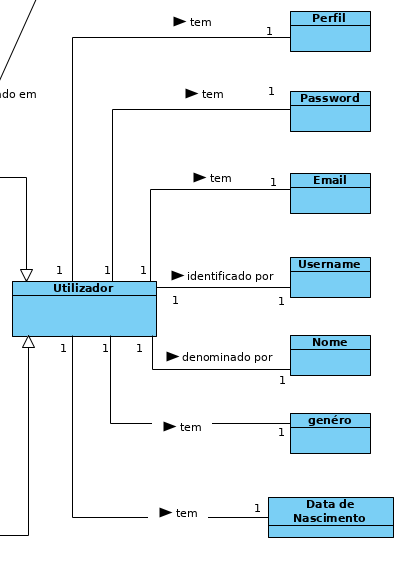
\includegraphics[scale=0.50]{images/modelação/utilizadores.png}
    \caption{Entidade Utilizador.}
    \label{fig:interfaceperfilptbycliente}
\end{figure}

\hspace{5mm} Tal como se pode observar a entidade \textbf{Utilizador} representa a informação comum a ambos os utilizadores, essa informação é: o \textbf{username} pelo qual o mesmo é identificado, o \textbf{nome} pelo qual é denominado, o \textbf{email} para pode ser contactado, a \textbf{password} que assegura a sua conta, o \textbf{género} e por última a sua \textbf{data de nascimento} (a partir da mesma pode ser derivada a sua idade). Juntamente com a informação referida e outras, específicas a cada utilizador (referidas adiante), o Utilizador contém um \textbf{perfil} que pode ser consultado por outros.

\hspace{5mm} Existem dois tipos de utilizadores: o \textbf{Cliente} e o \textbf{Personal Trainer}. De seguida seguinte encontra-se representado o Cliente.

\begin{figure}[H]
    \centering
    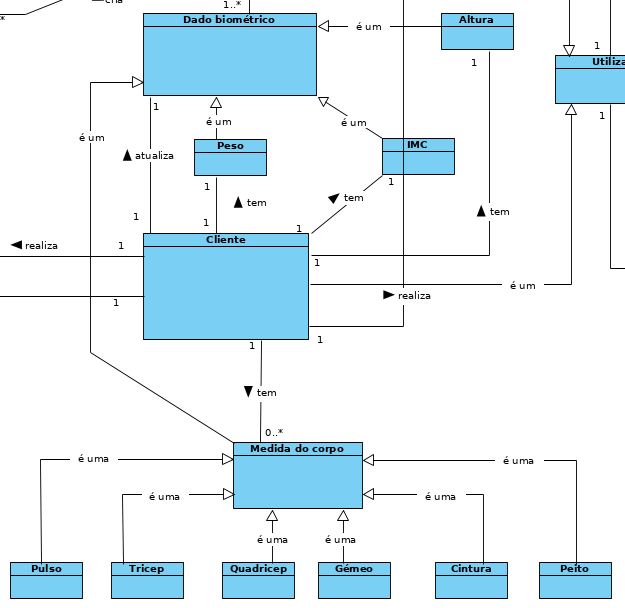
\includegraphics[scale=0.50]{images/modelação/cliente.png}
    \caption{Entidade Cliente.}
    \label{fig:interfaceperfilptbycliente}
\end{figure}

\hspace{5mm} O Cliente, a acrescentar à informação já referida, pode conter oito \textbf{dados biométricos}, sendo que as medidas: do \textbf{pulso, trícep, quadrícep, gémeo, cintura e peito} são dados opcionais, no entanto a introdução do \textbf{peso e altura} é obrigatória no momento de registo no sistema. O \textbf{IMC - Índice de Massa Corporal} - é derivado através de uma fórmula a partir do peso e altura sendo que as categorias (do IMC) que apresentamos no sistema seguem os dados fornecidos pela OMS - Organização Mundial de Saúde. Todos estes dados podem ser actualizados a qualquer momento e são sempre preservados os registos anteriores de modo a existir uma noção de histórico/ evolução. Note-se que apesar de opcionais, é recomendado a introdução de todos os dados uma vez que são métricas que permitem um acompanhamento mais personalizado e conclusivo sobre a evolução do plano de treino permitindo ajustar o plano consoante os resultados.

\hspace{5mm} O Personal Trainer é representado de seguida.

\begin{figure}[H]
    \centering
    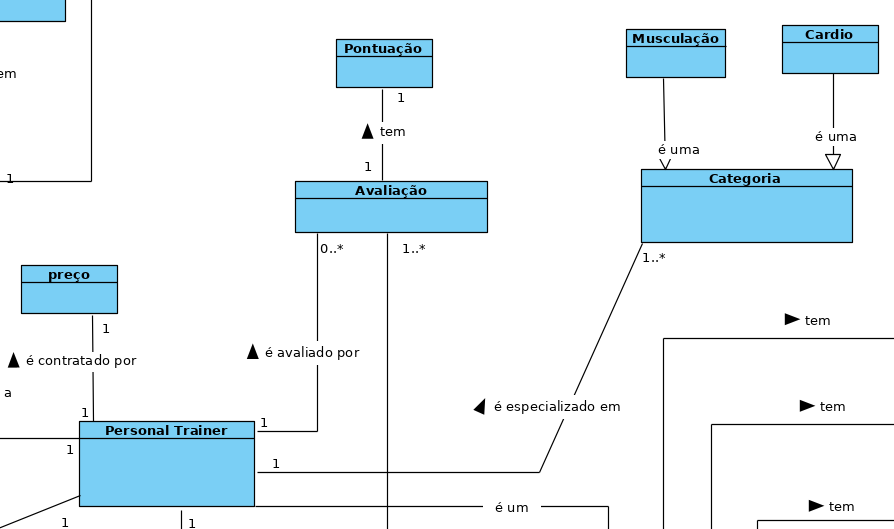
\includegraphics[scale=0.45]{images/modelação/pt.png}
    \caption{Entidade Personal Trainer.}
    \label{fig:interfaceperfilptbycliente}
\end{figure}

\hspace{5mm} Do mesmo modo, além da informação comum, contém também o \textbf{preço} que aplica ao Cliente por cada Workout (entidade explicada mais à frente), contém também a \textbf{categoria} em que é especializado, podendo ser em \textbf{musculação ou cardio}. Esta categoria pode ser útil quando o Cliente está a escolher o Personal Trainer que deseja ou mesmo pode ser útil ao próprio Personal Trainer para aceitar ou recusar um pedido de plano de treino uma vez que esse pedido pode não corresponder à sua categoria. A \textbf{avaliação} 
pode ser, também, decisiva no momento da escolha. Esta é realiza pelo Cliente uma única vez durante o plano de treino, numa escala de 1 a 5 estrelas (\textbf{pontuação}), sendo registada e associada às avaliações já existentes, calculando-se a média das mesmas.

\hspace{5mm} De seguida apresentam-se as entidades principais do modelo de negócio.

\begin{figure}[H]
    \centering
    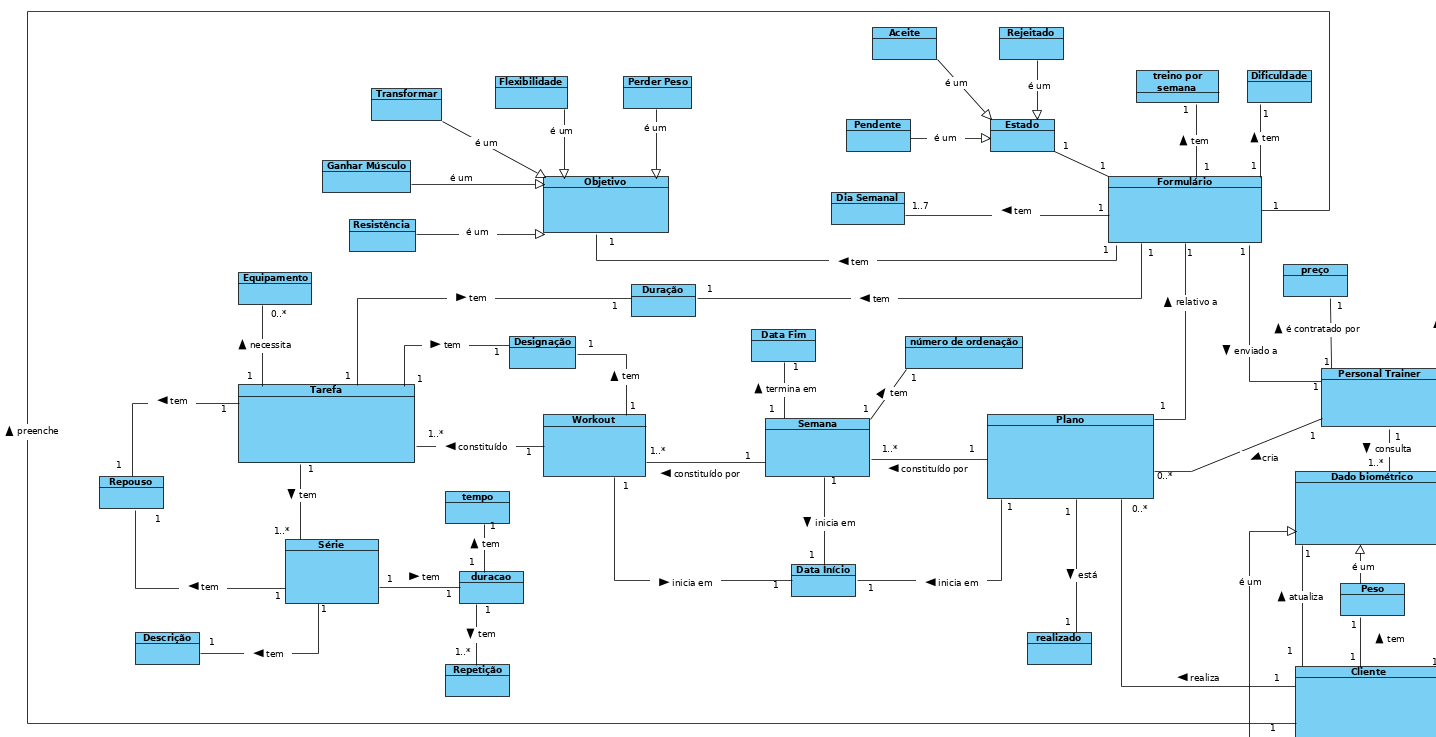
\includegraphics[scale=0.37]{images/modelação/core.png}
    \caption{Entidades principais do modelo de negócio.}
    \label{fig:interfaceperfilptbycliente}
\end{figure}

\hspace{5mm} Para iniciar um \textbf{plano} de treino, previamente, o Cliente tem de preencher um \textbf{formulário} onde indica a \textbf{dificuldade} que pode ser: \textbf{fácil, normal, difícil ou extrema}; é indicado também o número de \textbf{treinos semanais} juntamente com os \textbf{dias semanais} que tem disponibilidade, o \textbf{objectivo} que pode ser: \textbf{perder peso, ganhar músculo, resistência, flexibilidade e transformar gordura em massa magra}; e por último a \textbf{duração} em semanas.

\hspace{5mm} O formulário fica com o \textbf{estado pendente} até ao Personal Trainer o \textbf{rejeitar} ou \textbf{aceitar}. Caso o Personal Trainer aceite, imediatamente pode criar a primeira \textbf{semana} do \textbf{plano} de treino. 

\hspace{5mm} Uma semana ocorre entre duas datas: \textbf{data de início} e \textbf{data de fim}, contém também (internamente) o \textbf{número (de ordenação)} da semana no plano de treino. 

\hspace{5mm} A \textbf{semana} é constituída, também, por 1 ou mais \textbf{Workouts} que representa um dia de treino, por isso ocorre numa determinada \textbf{data} (num dia da semana), a \textbf{designação} que resume o treino nesse dia e a lista de \textbf{tarefas} a realizar.

\hspace{5mm} Uma \textbf{tarefa} contém, também, uma \textbf{designação}, uma \textbf{duração} (em minutos), pode necessitar de \textbf{equipamento} e as sucessivas tarefas são intervaladas por um \textbf{tempo de repouso}, por último é constituída por várias \textbf{séries}.

\hspace{5mm} A \textbf{série} é a unidade mais básica do plano de treino, contém uma \textbf{descrição} que indica a actividade a ser realizada. Tal como a tarefa, cada série é também intervalada com um \textbf{tempo de repouso}. Por último contém uma \textbf{duração} que pode ser em \textbf{tempo} (segundos ou minutos) ou em \textbf{número de repetições}. Para clarificar a noção de duração observe-se os seguintes exemplos: caso a série seja realizar 30 abdominais, a duração é 30 repetições, por outro lado, caso a série seja realizar a o movimento de prancha durante 1 minuto, a duração é em tempo (neste caso em minutos). 